\pdfoutput=1
\documentclass[a4paper,pdflatex,ja=standard]{bxjsarticle}

% ---Setting about the geometry of the document----
% \usepackage{a4wide}
% \pagestyle{empty}

% ---Physics and Math Packages---
\usepackage{amssymb,amsfonts,amsthm,mathtools}
\usepackage{physics,braket,bm}

% ---underline---
\usepackage{ulem}

% --- sorround the texts or equations
% \usepackage{fancybox,ascmac}

% ---settings of theorem environment---
% \usepackage{amsthm}
% \theoremstyle{definition}

% ---settings of proof environment---
% \renewcommand{\proofname}{\uline{\textbf{証明}}}
% \renewcommand{\qedsymbol}{$\blacksquare$}

% ---Ignore the Warnings---
\usepackage{silence}
\WarningFilter{latexfont}{Some font shapes,Font shape}

% ---Insert the figure (If insert the `draft' at the option, the process becomes faster)---
\usepackage{graphicx}
% \usepackage{subcaption}

% ----Add a link to a text---
\usepackage{url}
\usepackage{xcolor,hyperref}
\hypersetup{colorlinks=true,citecolor=orange,linkcolor=blue,urlcolor=magenta}
\usepackage{bxcjkjatype}

% ---Tikz---
\usepackage{tikz,pgf,pgfplots,circuitikz}
\pgfplotsset{compat=1.15}
\usetikzlibrary{intersections,arrows.meta,angles,calc,3d,decorations.pathmorphing}

% ---Add the section number to the equation, figure, and table number---
\makeatletter
   \renewcommand{\theequation}{\thesubsection.\arabic{equation}}
   \@addtoreset{equation}{subsection}
   
   \renewcommand{\thefigure}{\thesection.\arabic{figure}}
   \@addtoreset{figure}{section}
   
   \renewcommand{\thetable}{\thesection.\arabic{table}}
   \@addtoreset{table}{section}
\makeatother

% ---enumerate---
\renewcommand{\labelenumi}{\arabic{enumi}.}
\renewcommand{\labelenumii}{(\roman{enumii})}
\renewcommand{\labelenumiii}{(\alph{enumiii})}

% ---Index---
% \usepackage{makeidx}
% \makeindex

% ---Fonts---
\renewcommand{\familydefault}{\sfdefault}

% ---Title---
\title{東京大学\ 平成22年\ 物理学専攻\ 院試\ 解答例}
\author{ミヤネ}
\date{最終更新:\today}

\newcommand{\prb}[2]{
  \phantomsection
  \addcontentsline{toc}{subsection}{問題 #1: #2}
  \subsection*{第#1問\phantom{#2}}
  \setcounter{subsection}{#1}
  \setcounter{equation}{0}
}

\begin{document}

\maketitle

\tableofcontents
\clearpage


\section{数学パート}

\prb{1}{線形代数・微積分}

\begin{enumerate}

  \item 

  $f(\bm{x})$の停留点が$\bar{\bm{x}}$であることを確認しましょう.$x_i$で$f(\bm{x})$を微分してみると
  \begin{equation}
    \pdv{f(\bm{x})}{x_i}
    =
    \frac{1}{2}\sum_{j=1}^{n}A_{ij}x_j
    +
    \frac{1}{2}\sum_{j=1}^{n}x_jA_{ji}
    -
    b_i
    =
    \sum_{j=1}^{n}A_{ij}x_j
    -
    b_i
    \label{differential}
  \end{equation}
  となりますが,$\bm{x}=\bar{\bm{x}}$ならこの値は0になります.したがって,$\bm{x}=\bar{\bm{x}}$は停留点です.さらにヘッシアンですが,すべての点において
  \begin{equation}
    H
    =
    \begin{vmatrix}
      A_{11} & A_{12} & \cdots & A_{1n} \\
      A_{21} & A_{22} & \cdots & A_{2n} \\
      \vdots & \vdots & \ddots & \vdots \\
      A_{n1} & A_{n2} & \cdots & A_{nn}
    \end{vmatrix}
    =
    \det A
  \end{equation}
  であり,今は$A$の固有値は正なので,停留点はすべて極小.よって,$\bm{x}=\bar{\bm{x}}$は最小です.


  \item 

  \eqref{differential}で$\bm{x}=\bm{x}^{(m)}$を代入すれば
  \begin{equation}
    -\bm{r}
    =
    A\bm{x}^{(m)}-\bm{b}
  \end{equation}
  です.$\bm{b}=A\bar{\bm{x}}$を代入すれば,
  \begin{equation}
    \bm{r}
    =
    -A(\bm{x}^{(m)}-\bar{\bm{x}})
  \end{equation}
  となります.


  \item 

  $f(\bm{x}^{(m+1)})-f(\bm{x}^{(m)})$が最も大きくなるような$\alpha$を選べばよいでしょう.計算してみると
  \begin{align}
    f(\bm{x}^{(m+1)})-f(\bm{x}^{(m)})
    &=
    \frac{1}{2}
    (\bm{x}^{(m)}+\alpha\bm{r})^{T}A(\bm{x}^{(m)}+\alpha\bm{r})
    -
    \bm{b}^{T}(\bm{x}^{(m)}+\alpha\bm{r})
    \nonumber
    \\
    &\hspace{5cm}
    -
    \frac{1}{2}{\bm{x}^{(m)}}^{T}A\bm{x}^{(m)}
    +
    \bm{b}^{T}\bm{x}^{(m)}
    \nonumber
    \\
    &=
    \underbrace{
      \alpha{\bm{x}^{(m)}}^{T}A\bm{r}
      -
      \alpha\bm{b}^{T}\bm{r}
    }_{=-\alpha\bm{r}^{T}\bm{r}}
    +
    \frac{\alpha^2}{2}\bm{r}^{T}A\bm{r}
    \nonumber
    \\
    &=
    \frac{\|\bm{r}\|_{A}^2}{2}
    \left(  
      \alpha-\frac{\|\bm{r}\|^2}{\|\bm{r}\|_{A}^2}
    \right)^2
    -
    \frac{\|\bm{r}\|^4}{2\|\bm{r}\|_{A}^2}
  \end{align}
  となるので,この値が最も小さくなるのは$\alpha=\|\bm{r}\|^2/\|\bm{r}\|_{A}^2$のときです.


  \item 

  $\delta\bm{x}^{(m+1)}=\bm{x^{m}}+\alpha\bm{r}-\bar{\bm{x}}=\delta\bm{x}^{(m)}+\alpha\bm{r}$なので,
  \begin{align}
    \|\delta\bm{x}^{(m+1)}\|_A^2
    &=
    (\delta\bm{x}^{(m)}+\alpha\bm{r})^{T}A(\delta\bm{x}^{(m)}+\alpha\bm{r})
    \nonumber
    \\
    &=
    \|\delta\bm{x}^{(m)}\|_{A}^2
    +
    \alpha^2\|\bm{r}\|_{A}^2
    +
    \alpha(\bm{r}^TA\delta\bm{x}^{(m)}+{\delta\bm{x}^{(m)}}^{T}A\bm{r})
  \end{align}
  です.最後の項については
  \begin{equation}
    \delta\bm{x}^{(m)}
    =
    \bm{x}^{(m)}-\bar{\bm{x}}
    =
    -A^{-1}\bm{r}
  \end{equation}
  なので,$\bm{r}^TA\delta\bm{x}^{(m)}+{\delta\bm{x}^{(m)}}^{T}A\bm{r}=-2\|\bm{r}\|^2$となります.よって,最後に$\alpha$を代入すれば
  \begin{equation}    
    \|\delta\bm{x}^{(m+1)}\|_A
    =
    \sqrt{
      \|\delta\bm{x}^{(m)}\|_{A}^2
      -
      \frac{\|\bm{r}\|^4}{\|\bm{r}\|_A^2}
    }
  \end{equation}
  です.


  \item 

  前問の結果より
  \begin{equation}
    R
    =
    \sqrt{
      1
      -
      \frac{1}{\|\delta\bm{x}^{(m)}\|_{A}^2}
      \frac{\|\bm{r}\|^4}{\|\bm{r}\|_A^2}      
    }
  \end{equation}
  を計算します.それぞれの因子は
  \begin{align}
    \|\delta\bm{x}^{(m)}\|_{A}^2
    &=
    {\delta\bm{x}^{(m)}}^T
    A
    \delta\bm{x}^{(m)}
    \nonumber
    \\
    &=
    \left( \sum_{j=1}^{n}\rho_j\bm{a}_j^T \right)
    \left( \sum_{i=1}^{n}\lambda_i\rho_i\bm{a}_i \right)
    =
    \sum_{i=1}^{n}
    \lambda_i\rho_i^2
    \\
    \|\bm{r}\|^2
    &=
    \|A\delta\bm{x}^{(m)}\|^2
    \nonumber
    \\
    &=
    \left( \sum_{j=1}^{n}\lambda_j\rho_j\bm{a}_j^T \right)
    \left( \sum_{i=1}^{n}\lambda_i\rho_i\bm{a}_i \right)
    \nonumber
    \\
    &=
    \sum_{i=1}^{n}
    \lambda_i^2\rho_i^2
    \\    
    \|A\delta\bm{x}^{(m)}\|_A^2
    &=
    \left( \sum_{j=1}^{n}\lambda_j\rho_j\bm{a}_j^T \right)
    \left( \sum_{i=1}^{n}\lambda_i^2\rho_i\bm{a}_i \right)    
    \nonumber
    \\
    &=
    \sum_{i=1}^{n}
    \lambda_i^3\rho_i^2
  \end{align}
  となるので,
  \begin{equation}
    R
    =
    \sqrt{
      1
      -
      \dfrac{{\displaystyle \left( \sum_{i=1}^{n}
      \lambda_i^2\rho_i^2 \right)^2}}{{ \displaystyle
        \left( 
          \sum_{i=1}^{n}
          \lambda_i\rho_i^2 \right)
        \left( 
          \sum_{i=1}^{n}
          \lambda_i^3\rho_i^2 \right)}
      }
    }
  \end{equation}
  です.


  \item 

  前問の総和が$i=1,2$で行われることに注意すれば
  \begin{equation}
    R
    =
    \sqrt{
      1
      -
      \dfrac{
        \left( \rho_1^2p^2+\rho_2^2 \right)^2
      }{
        \left( \rho_1^2 p+\rho_2^2 \right)
        \left( \rho_1^2p^3+\rho_2^2 \right)
      }
    }
  \end{equation}
  となりますが,$0<p\leq1$より
  \begin{equation}
    \sqrt{
      1
      -
      \dfrac{
        \left( \rho_1^2p^2+\rho_2^2 \right)^2
      }{
        \left( \rho_1^2 p+\rho_2^2 \right)
        \left( \rho_1^2p^3+\rho_2^2 \right)
      }
    }
    <    
    \sqrt{
      1
      -
      \dfrac{
        \rho_2^4
      }{
        \left( \rho_1^2+\rho_2^2 \right)^2
      }
    }
    \equiv
    A
    \ 
    (<1)
  \end{equation}
  です\footnote{
    分母は$p=0$,分子は$p=1$で不等式をつくりました.
  }.したがって,$\|\delta\bm{x}^{(m+1)}\|=A\|\delta\bm{x}^{(m)}\|$なので,$m\rightarrow\infty$で$\|\delta\bm{x}^{(m)}\|_A\rightarrow0$となり,$\bm{x}^{(m)}\rightarrow\bar{\bm{x}}$です.


\end{enumerate}



\clearpage

\prb{2}{微分方程式}

\begin{enumerate}
  
  \item 

  微分の変換は
  \begin{equation}
    \begin{pmatrix}
      \pdv{}{t} \\
      \pdv{}{x}
    \end{pmatrix}
    =
    \begin{pmatrix}
      v\pdv{}{\xi}-v\pdv{}{\eta} \\
      \pdv{}{\xi}+\pdv{}{\eta}
    \end{pmatrix}
    =
    \begin{pmatrix}
      v & -v \\
      1 & 1
    \end{pmatrix}
    \begin{pmatrix}
      \pdv{}{\xi} \\
      \pdv{}{\eta}
    \end{pmatrix}
  \end{equation}
  です.よって,
  \begin{align}
    \frac{1}{v^2}
    \pdv[2]{u}{t}
    -
    \pdv[2]{u}{x}
    &=
    \frac{1}{v^2}
    \left(  
      v\pdv{}{\xi}-v\pdv{}{\eta}
    \right)^2
    u
    -
    \left( \pdv{}{\xi}+\pdv{}{\eta} \right)^2
    u
    \nonumber
    \\
    &=
    -4\pdv{u}{\xi}{\eta}
  \end{align}
  より,$u(x,t)$が満たす方程式は
  \begin{equation}
    \pdv{u}{\xi}{\eta}
    =
    0
    \label{diffeq}
  \end{equation}
  です.


  \item 

  $f(\xi)$や$g(\eta)$は\eqref{diffeq}を満たしています.その線形結合も解です.
  

  \item 

  $t$に依存しないことを示すためには,$t$で微分してみるとよいでしょう.実際
  \begin{align}
    \pdv{I}{t}
    &=
    \frac{1}{2}
    \int_{-\infty}^{+\infty}
    \left[  
      \frac{2}{v^2}
      \pdv{u}{t}\pdv[2]{u}{t}
      +
      2\pdv{u}{x}\pdv{u}{x}{t}
    \right]
    \dd x
    \nonumber
    \\
    &=    
    \left[  
      \pdv{u}{x}\pdv{u}{t}
    \right]_{-\infty}^{+\infty}
    +
    \int_{-\infty}^{+\infty}
    \left[  
      \frac{1}{v^2}
      \pdv{u}{t}\pdv[2]{u}{t}
      -
      \pdv[2]{u}{x}\pdv{u}{t}
    \right]
    \dd x
    \nonumber
    \\
    &=
    0
    +
    \int_{-\infty}^{+\infty}
    \pdv{u}{x}
    \left[  
      \frac{1}{v^2}
      \pdv[2]{u}{t}
      -
      \pdv[2]{u}{x}
    \right]
    \dd x
    =
    0
  \end{align}
  です.


  \item 

  初期条件を$f,g$で書くと
  \begin{equation}
    f(x)+g(x)
    =
    u_0(x)
    ,\ 
    vf'(x)-vg'(x)
    =
    u_1(x)
  \end{equation}
  です.したがって,
  \begin{equation}
    f(x)
    =
    \frac{1}{2}u_0(x)
    +
    \frac{1}{2v}\int_{0}^{x} u_1(y)\dd y
    ,\ 
    g(x)
    =
    \frac{1}{2}u_0(x)
    -
    \frac{1}{2v}\int_{0}^{x} u_1(y)\dd y
  \end{equation}
  となるので,
  \begin{equation}
    u(x,t)
    =
    \frac{u_{0}(x+vt)+u_{0}(x-vt)}{2}
    +
    \frac{1}{2v}\int_{x-vt}^{x+vt}u_1(y)\dd y
  \end{equation}
  が求める解です.


  \item 

  前問の結果に代入すれば
  \begin{equation}
    u(x,t)
    =
    \frac{vb}{2\pi}
    \int_{x-vt}^{x+vt}
    \frac{\dd y}{(y-a)^2+b^2}
  \end{equation}
  となります.積分は$z\equiv (y-a)/b$と変数変換すれば
  \begin{equation}
    \int_{x-vt}^{x+vt}
    \frac{\dd y}{(y-a)^2+b^2}
    =
    \frac{1}{b}
    \int_{z_{-}}^{z_{+}}
    \frac{\dd z}{z^2+1}
  \end{equation}
  となります.ただし
  \begin{equation}
    z_{\pm}
    \equiv
    \frac{x\pm vt-a}{b}
  \end{equation}
  とおきました.よって,
  \begin{equation}    
    \int_{z_{-}}^{z_{+}}
    \frac{\dd z}{z^2+1}
    =
    \tan^{-1}z_{+}
    -
    \tan^{-1}z_{-}
    =
    \tan^{-1}
    \frac{x+vt-a}{b}
    -
    \tan^{-1}
    \frac{x-vt-a}{b} 
  \end{equation}
  となるので
  \begin{equation}
    u(x,t)
    =
    \frac{v}{2\pi}
    \left[  
      \tan^{-1}
      \frac{x+vt-a}{b}
      -
      \tan^{-1}
      \frac{x-vt-a}{b}       
    \right]
  \end{equation}
  です.ここで,次の公式
  \begin{equation}
    \tan^{-1}\alpha
    -
    \tan^{-1}\beta
    =
    \tan^{-1}
    \frac{\alpha-\beta}{1+\alpha\beta}
  \end{equation}
  を用いれば
  \begin{equation}
    \tan^{-1}
    \frac{x+vt-a}{b}
    -
    \tan^{-1}
    \frac{x-vt-a}{b}   
    =
    \tan^{-1}
    \cfrac{2vt/b}{1+\cfrac{(x-a)^2-v^2t^2}{b^2}}    
  \end{equation}
  なので
  \begin{equation}
    u(x,t)
    =
    \frac{v}{2\pi}
    \tan^{-1}
    \frac{2bvt}{(x-a)^2-v^2t^2+b^2}
  \end{equation}
  が求める解となります.


  \item 

  $b\rightarrow0$の極限では,$b^2$の寄与が無視できて
  \begin{equation}
    u(x,t)
    \sim
    \frac{v}{2\pi}
    \tan^{-1}
    \frac{2bvt}{(x-a)^2-v^2t^2}
  \end{equation}
  となります.(概形は省略します.$x=a$で負のピークをもつ形になるでしょう.)


\end{enumerate}




\clearpage

\section{物理パート}

\prb{1}{量子力学}

\begin{enumerate}

  \item 

  $-L\leq x\leq L$でのシュレーディンガー方程式は
  \begin{equation}
    \psi(x)
    =
    -k^2\psi(x)
    ,\ 
    k\equiv \sqrt{\frac{2mE}{\hbar^2}}
  \end{equation}
  なので,その解は
  \begin{equation}
    \psi(x)
    =
    A\sin kx
    +
    B\cos kx
  \end{equation}
  と書けます.境界条件は$\psi(L)=0$なので
  \begin{equation}
    A\sin k_n L+B\cos k_n L
    =
    0
  \end{equation}
  となり,$A=0\ \mathrm{or}\ B=0$です.それぞれの場合を考えると
  \begin{equation}
    \left\{
      \begin{alignedat}{1}
        A=0\text{のとき}
        \ &\ 
        \cos k_nL=0\ \rightarrow\ 
        k_nL
        =
        \left( n-\frac{1}{2} \right)\pi
        \\
        B=0\text{のとき}
        \ &\ 
        \sin k_nL=0\ \rightarrow\ 
        k_nL
        =
        n\pi
      \end{alignedat}
    \right.
  \end{equation}
  となるので\footnote{
    このとき,$\psi(-L)=0$も成立しています.
  },エネルギー固有値は
  \begin{equation}
    E_{n}
    =
    \left\{
      \begin{alignedat}{1}
        \frac{\pi^2\hbar^2}{2mL^2}\left( n-\frac{1}{2} \right)^2
        \ &\ 
        \left( \psi(x)=\frac{1}{\sqrt{L}}\cos k_n x \right)
        \\
        \frac{\pi^2\hbar^2}{2mL^2}n^2
        \ &\ 
        \left( \psi(x)=\frac{1}{\sqrt{L}}\sin k_n x \right)
      \end{alignedat}
    \right.
  \end{equation}
  となります.ただし,$n=1,2,\cdots$です.


  \item 

  不確定性原理より$\Delta p\neq0$なので,粒子が運動量を持っている可能性があります.


  \item 

  無摂動の基底状態は
  \begin{equation}
    \psi_0(x)
    =
    \frac{1}{\sqrt{L}}\cos\left( \frac{\pi}{2L}x \right)
  \end{equation}
  なので
  \begin{equation}
    E_0^{(1)}
    =
    \mel*{\psi_0}{\Delta V}{\psi_0}
    =
    \frac{1}{L}
    \int_{-L}^{L}
    V_1\delta(x)\cos^2\left( \frac{\pi}{2L}x \right)
    \dd x
    =
    \frac{1}{L}V_1
  \end{equation}
  です.(ただし,$\Delta V\equiv V_1\delta(x)$とおきました.)よって,
  \begin{equation}
    E_0
    \sim
    \frac{\pi^2\hbar^2}{8mL}
    +
    \frac{1}{L}V_1
    \label{ans_2_1_3}
  \end{equation}
  となります.


  \item 

  第1励起状態の無摂動の波動関数は
  \begin{equation}
    \psi_1(x)
    =
    \frac{1}{\sqrt{L}}
    \sin\left( \frac{\pi}{L}x \right)
  \end{equation}
  なので,摂動の1次は0です.波動関数が$\sin$型で,ポテンシャルが$x=0$のみに値を持つので,摂動はなくなります\footnote{
    この摂動の計算では
    $$
      \int_{-L}^{L}
      \psi_k^{*}(x)\times V_1\delta(x)\sin\left( \frac{\pi}{L}x \right)
      \dd x
      =
      \psi_{k}^{*}(0)\times V_1\sin 0
      =
      0
    $$
    といった因子が必ず入ってくるので,0になります.($\psi_{k}(x)$は第$k$励起状態です.)
  }.したがって,
  \begin{equation}
    E_1
    =
    \frac{\pi^2\hbar^2}{2mL^2}
  \end{equation}
  のままです.


  \item 
  
  図\ref{ans_2_1_5}のようになります.

  \begin{figure}[ht]
    \centering    
    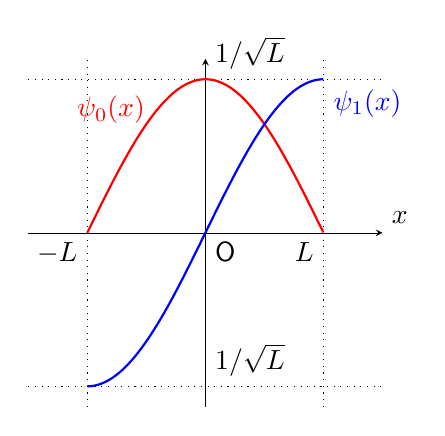
\begin{tikzpicture}[xscale=1.5, yscale=1.3]
      \draw[->,>=stealth,ultra thin](0,-1.7)--(0,1.7);
      \draw[->,>=stealth,ultra thin](-1.5,0)--(1.5,0)node[above right]{$x$};
      \draw[dotted,thin](1,-1.7)--(1,1.7);
      \draw[dotted,thin](-1,-1.7)--(-1,1.7);
      \draw[dotted,thin](-1.5,-1.5)--(1.5,-1.5);
      \draw[dotted,thin](-1.5,1.5)--(1.5,1.5);
      \draw(0,0)node[below right]{O};
      \draw(1,0)node[below left]{$L$};
      \draw(-1,0)node[below left]{$-L$};
      \draw[samples=100,domain=-1:1,thick, red]plot(\x,{1.5*(cos(\x*90))}); 
      \draw[samples=100,domain=-1:1,thick, blue]plot(\x,{1.5*(sin(\x*90))}) node[below right]{$\psi_1(x)$}; 
      \draw[red](-0.8,1.2)node{$\psi_0(x)$};
      \draw(0,1.5)node[above right]{$1/\sqrt{L}$};
      \draw(0,-1.5)node[above right]{$1/\sqrt{L}$};
    \end{tikzpicture}
    \caption{$\psi_0(x)$と$\psi_1(x)$の概形}
    \label{ans_2_1_5}
  \end{figure}


  \item 
  $V_1$が$E_0^{(0)}$に比べて非常に小さいときは\eqref{ans_2_1_6}のようになり,これは$E_1$を超えないように上昇すると考えられます.(一方で$E_1$は変化しません.)したがって,図\ref{ans_2_1_6}のようになると考えられます.

  \begin{figure}[ht]
    \centering    
    \begin{tikzpicture}[scale=2.0]
      \draw[->,>=stealth,ultra thin](0,-0.3)--(0,1.8);
      \draw[->,>=stealth,ultra thin](-0.3,0)--(2.0,0)node[below right]{$V_1$};
      \draw[dotted,thin](-0.3,1.5)--(2.0,1.5)node[right]{$E_1$};
      \draw[samples=100, domain=0.0:2.0, thick]plot(\x,{1.4-exp(-2*\x)});
      \draw(0.9,1.0) node{$E_0$};
    \end{tikzpicture}
    \caption{$E_0$と$E_1$}
    \label{ans_2_1_6}
  \end{figure}


\end{enumerate}



\clearpage

\prb{2}{統計力学}

\begin{enumerate}

  \item 

  状態数は
  \begin{equation}
    W
    =
    \frac{(N_{\alpha}+N_{\beta})!}{N_{\alpha}!N_{\beta}!}
  \end{equation}
  なので,ボルツマンの法則より
  \begin{equation}
    S
    =
    k_B
    \log W
    =
    k_B
    \left( \log(N_{\alpha}+N_{\beta})!-\log N_A!-\log N_B! \right)
  \end{equation}
  です.


  \item 

  前問の結果を$N$で割って,スターリングの公式を用いれば
  \begin{align}
    s
    &=
    k_B
    \left[  
      \left( \frac{N_{\alpha}}{N}+\frac{N_{\beta}}{N} \right)
      \log(N_{\alpha}+N_{\beta})
      -
      \frac{N_{\alpha}}{N}\log N_{\alpha}
      -
      \frac{N_{\beta}}{N}\log N_{\beta}
    \right]
    \nonumber
    \\
    &=
    k_B
    \left[  
      \frac{N_{\alpha}}{N}
      \log\left( 1+\frac{N_{\beta}}{N_{\alpha}} \right)
      +
      \frac{N_{\beta}}{N}
      \log\left( 1+\frac{N_{\alpha}}{N_{\beta}} \right)
    \right]
    \label{entropy_per_mol}
  \end{align}
  となります.ここで,次の2式
  \begin{equation}
    \frac{N_{\alpha}}{N}
    +
    \frac{N_{\beta}}{N}
    =
    1
    ,\ 
    \varepsilon
    =
    -f\left( a\frac{N_{\alpha}}{N}+b\frac{N_{\beta}}{N} \right)
  \end{equation}
  を解けば
  \begin{equation}
    \frac{N_{\alpha}}{N}
    =
    -\frac{\varepsilon+bf}{f(a-b)}
    ,\ 
    \frac{N_{\beta}}{N}
    =
    \frac{\varepsilon+af}{f(a-b)}
  \end{equation}
  となるので,\eqref{entropy_per_mol}に代入すれば
  \begin{equation}
    s
    =
    -
    \frac{k_B}{f(a-b)}
    \left[  
      (\varepsilon+bf)\log\frac{f(b-a)}{\varepsilon+bf}
      -
      (\varepsilon+af)\log\frac{f(a-b)}{\varepsilon+af}
    \right]
    \label{ans2_2_2_func}
  \end{equation}
  となります.

  エントロピーの概形ですが,\eqref{ans2_2_2_func}は$b-a<0$より実は定義不可能です.したがって,物理的な解釈から書いてあげるのがよいかと思います.まず,$\varepsilon$の絶対値が最小値に近ければ近いほど,系は$N_{\alpha}\sim 1,\ N_{\beta}\sim 0$となっていきます.すると,状態数が小さくなるので,エントロピーも小さくなっていると考えられます.そこから$\varepsilon$の絶対値が大きくなると,系のとれる状態数がだんだん大きくなっていき,あるピークを超えると今度は$N_{\alpha}\sim 0,\ N_{\beta}\sim 1$という状態に近づき,エントロピーは再び減少していくはずです.以上のことを踏まえると,図\ref{ans_2_2_2}のように変化すると考えられます.

  \begin{figure}[ht]
    \centering    
    \begin{tikzpicture}[scale=2.0]
      \draw[->,>=stealth,ultra thin](0,-0.3)--(0,2.0)node[left]{$s$};
      \draw[->,>=stealth,ultra thin](-0.3,0)--(2.0,0)node[below right]{$|\varepsilon|$};
      \draw[samples=100, domain=0.5:1.5, thick]plot(\x,{1.6*sin(180*(\x-0.5))});     
      \draw(0.5,0)node[below]{$fa$};  
      \draw(1.5,0)node[below]{$fb$};  
    \end{tikzpicture}
    \caption{エネルギーの絶対値$|\varepsilon|$とエントロピー$s$の関係}
    \label{ans_2_2_2}
  \end{figure}


  \item 

  分配関数は,粒子が$\alpha$か$\beta$の状態しか取れないことに注意すれば
  \begin{equation}
    Z[\beta]
    =
    \sum_{\sigma=\alpha,\beta}e^{-\beta \varepsilon_{\sigma}}
    =
    e^{\beta fa}
    +
    e^{\beta fb}
  \end{equation}
  となります.したがって,自由エネルギーは
  \begin{equation}
    F[T]
    =
    -\frac{1}{\beta}\log Z
    =
    -k_BT\log 
    \left[ 
      e^{fa/k_BT}
      +
      e^{fb/k_BT} 
    \right]
  \end{equation}
  なので,エントロピーは
  \begin{align}
    s
    &=
    -\pdv{F}{T}
    \nonumber
    \\
    &=
    k_B\log(e^{fa/k_BT}+e^{fb/k_BT})
    -
    \frac{f}{T}\frac{ae^{fa/k_BT}+be^{fb/k_BT}}{e^{fa/k_BT}+e^{fb/k_BT}}
  \end{align}
  となります.$T\rightarrow0$では,$a>b$より$e^{fa/k_BT}$の寄与が大きいと考えられるので
  \begin{equation}
    s
    \rightarrow
    \frac{fa}{T}
    -
    \frac{f}{T}
    \frac{ae^{fa/k_BT}}{e^{fa/k_BT}}
    =
    0
  \end{equation}
  です.一方で$T\rightarrow\infty$では,$e^{fa/k_BT},\ e^{fb/k_BT}\rightarrow1$より
  \begin{equation}
    s
    \rightarrow
    k_B \log 2
    \label{ans_Tinfinity}
  \end{equation}
  となります.


  \item 

  温度が小さければ小さいほど$e^{fa/k_BT}\gg e^{fb/k_BT}$となることから,長さの値が大きくなると考えられます.したがって,逆に考えれば,温度が大きくなればなるほど,状態$\beta$になる粒子が多くなるので,鎖は\uline{短くなる}と考えられます.

  $T=0$では,すべての粒子が状態$\alpha$にあると考えられるので,単量体1つあたり$l(0)=a$です.一方で,$T=\infty$では,$e^{fa/k_BT}\sim e^{fb/k_BT}\sim 1$より,状態$\alpha$と状態$\beta$の粒子が半々で存在する\footnote{
    前問の答え\eqref{ans_Tinfinity}もこの考え方と一致しています.
  }と考えられるので$l(\infty)=(a+b)/2$となります.


  \item
  
  \begin{equation}
    \int_{0}^{\infty}
    \frac{c(T)}{T}
    \dd T
    =
    s(\infty)-s(0)
    =
    k_B\log 2
    .
  \end{equation}


  \item 

  状態$\alpha$と状態$\beta$は等確率で存在すると考えられるので,$(a+b)/2$でしょう.


\end{enumerate}


\clearpage

\prb{3}{電磁気学}

\begin{enumerate}

  \item 

  磁場も$\bm{B}(\bm{r},t)=\bm{B}(\bm{r})e^{-i\omega t}$と書けるとすれば,マクスウェル方程式で
  \begin{equation}
    \pdv{}{t}
    \rightarrow
    -i\omega
  \end{equation}
  とするだけです.


  \item 

  前問の結果をまとめると,マクスウェル方程式は
  \begin{gather}
    \bm{\nabla}
    \cdot
    \bm{H}(\bm{r})
    =
    0
    \label{mag_zero}
    \\
    \bm{\nabla}
    \times
    \bm{E}(\bm{r})
    -
    i\omega\mu\bm{H}(\bm{r})
    =
    \bm{0}
    \label{faraday}
    \\
    \bm{\nabla}\cdot\bm{E}(\bm{r})
    =
    \frac{1}{\varepsilon}\rho(\bm{r})
    \label{gauss}
    \\
    \bm{\nabla}
    \times
    \bm{H}(\bm{r})
    +
    i\omega\varepsilon
    \bm{E}(\bm{r})
    =
    \bm{J}(\bm{r})
    \label{ampere}
  \end{gather}
  です.$\bm{E}$と$\bm{H}$の方程式を導出するためには,\eqref{faraday}と\eqref{ampere}の$\mathrm{rot}$をとればよいです.\eqref{faraday}のほうは
  \begin{equation}
    \bm{\nabla}(\bm{\nabla}\cdot\bm{E})
    -
    \bm{\nabla}^2\bm{E}
    -
    i\omega
    \left(  
      -
      i\omega\varepsilon\bm{E}
      +
      \bm{J}
    \right)
    =
    \bm{0}
  \end{equation}
  となるので,これを整理すれば
  \begin{equation}
    (\bm{\nabla}^2+\varepsilon\mu\omega^2)
    \bm{E}(\bm{r})
    -
    \frac{1}{\varepsilon}\bm{\nabla}\rho(\bm{r})
    +
    i\omega\bm{J}(\bm{r})
    =
    0
  \end{equation}
  となります.\eqref{ampere}のほうの$\mathrm{rot}$をとって整理すれば
  \begin{equation}
    (\bm{\nabla}^2+\varepsilon\mu\omega^2)
    \bm{H}(\bm{r})
    +
    \bm{\nabla}\times\bm{H}(\bm{r})
    =
    0
  \end{equation}
  です.


  \item 

  \eqref{faraday}に解を代入すれば
  \begin{equation}
    ik\bm{s}\times\bm{E}_0
    =
    i\mu\omega\bm{H}_0
    \label{faraday2}
  \end{equation}
  となるので,$\bm{H}_0\perp\bm{s},\ \bm{E}_0\perp\bm{H}_0$です.同様にして,\eqref{ampere}に解を代入すれば
  \begin{equation}
    ik\bm{s}\times\bm{H}_0
    =
    (\sigma-i\varepsilon\omega)\bm{E}_0
    \label{ampere2}
  \end{equation}
  となるので,$\bm{E}_0\perp\bm{s}$が分かります.


  \item 

  前問の2式\eqref{faraday2},\eqref{ampere2}の絶対値をとれば
  \begin{equation}
    \frac{|\bm{E}|}{|\bm{H}|}
    =
    \sqrt{\frac{\mu}{\varepsilon}}
  \end{equation}
  です.$\sigma\neq 0$のときは,そもそも波数が異なってくるので電場と磁場の位相がずれます.


  \item 

  完全導体の境界条件は「接線方向の電場が0」なので\footnote{
    一般に,電場と磁場の境界条件は
    $$
      (\bm{E}_1-\bm{E}_2)\cdot\bm{t}
      =
      0
      ,\ 
      (\bm{H}_1-\bm{H}_2)\cdot\bm{t}
      =
      \bm{J}\cdot\bm{t}
    $$
    です.今回は,完全導体内は電場が存在しないことから,境界条件を満たすためには接線方向の電場が0であることが必要です.
  },$y$軸方向に電場が振動し,それに垂直な$x$軸方向に磁場が振動します.


  \item 

  $xy$平面を一周する経路$\gamma$を考えれば,アンペールの法則より
  \begin{equation}
    I=\int_{\gamma}\bm{H}\cdot\dd\bm{l}
    =
    2b|\bm{H}_0|e^{ikz}
  \end{equation}
  です.


  \item 

  $z=z_0$における電位差は
  \begin{equation}
    V
    =
    -\int_{0}^{b}
    \bm{E}\cdot\dd\bm{l}
    =
    b|\bm{E}_0|e^{ikz_0}
  \end{equation}
  です.したがって,
  \begin{equation}
    \frac{V}{I}
    =
    \frac{|\bm{H}_0|}{2{\bm{E}_0}}
    =
    \frac{1}{2}\sqrt{\frac{\mu}{\varepsilon}}
  \end{equation}
  です.


\end{enumerate}


\end{document}
